\documentclass[3p,times,authoryear]{elsarticle}
\usepackage{amsmath,amssymb,amsthm,booktabs,array,tabularx}
\usepackage{graphicx,url,xcolor}
\usepackage{tikz}
\usetikzlibrary{arrows.meta,positioning}
\usepackage[hidelinks]{hyperref}
\newtheorem{lemma}{Lemma}
\newtheorem{proposition}{Proposition}
\renewcommand{\qedsymbol}{}
\newcommand{\ind}[1]{\mathbf{1}[#1]}
\newcommand{\NULL}{\mathrm{NULL}}
\newcommand{\ite}{\operatorname{If}}
\newcommand{\sat}{\textsc{sat}}
\newcommand{\unsat}{\textsc{unsat}}
\journal{Data \& Knowledge Engineering}
\begin{document}
\begin{frontmatter}
\title{CaliberGraph: Join-Multiplicity Encodings and Semantic Boundaries in Bounded SQL Verification}
\author{Hongsheng Wang}
\author{Dazhen Deng}
\begin{abstract}
Bounded SQL verification depends on both relational encodings and faithful translation of a database contract. We study these boundaries in CaliberGraph, an implementation of known join-multiplicity factorization for scalar SUM and COUNT over separable inner-star joins. Assignment-wise derivations establish the abstract product and finite-selector identities; a separate adapter audits a narrow integrity-constraint AST. Across 28 exposed configurations, six cost arms return 127 strictly accepted decisions in 168 slots. Flat obtains 23 strict results and selector 22; median costs and a cheap conjunction-normalization control establish no selector-specific benefit. A cached-AST scan admits six of 48,910 public query slots, all without joins. A separate ten-pair natural-query development inventory exposes a broader SQLite boundary. Resource-adapted Polygon runs on four admitted pairs yield two concrete inequivalences and two bounded UNSAT outcomes; eight synthetic databases distinguish three further pairs, and two inputs are invalid. A 42-case COUNT regression records three engineering repairs without claiming full-pipeline verification. These experiments separate abstract identities, frontend admission, concrete refutation and bounded absence of counterexamples. They support a restricted implementation and reproducible diagnostic findings, but do not establish a new encoding mechanism, general SQL correctness or comparative performance advantage.
\end{abstract}
\begin{keyword}
SQL equivalence \sep bounded verification \sep bag semantics \sep scalar aggregation \sep SMT encoding
\end{keyword}
\end{frontmatter}

\noindent\textit{Author-review candidate, 12 October 2026.} Author metadata and declarations remain subject to confirmation. This local candidate has not been submitted.

\section{Introduction}
Nullable arguments distinguish \texttt{COUNT(x)} from \texttt{COUNT(*)}; duplicate joins multiply measures; empty scalar SUM returns NULL. Testing one database can miss these differences. Bounded equivalence verification instead searches a declared tuple domain under supplied constraints, as implemented for complex SQL by VeriEQL \citep{he2024verieql}.

For a root tuple joined independently to several leaves, exact leaf-match counts multiply its contribution. We implement this known factorization as a product and compare a selector that substitutes guarded constant multiples with shared variables. Selectors remove one source of variable multiplication but add branches; measures and ICs can remain nonlinear. Benefits must survive known-factorization and preprocessing controls, including frontend, fallback and witness-checking costs.

Our object is fixed-query verification over a constructed INT-schema star fragment, not end-to-end NL2Metric or business-intent certification. Earlier CaliberGraph metadata scores do not validate it. We provide assignment-wise derivations, code using official base variables, a narrow contract-AST adapter and failure-preserving evidence. None certifies the text parser or the complete implementation. Public eligible pairs contain no join. A separate source-traceable development inventory therefore examines which barriers are frontend restrictions, semantic mismatches, or bounded-search outcomes. It does not retroactively enlarge the original fragment or provide an independent test set. Sections~\ref{sec:related}--\ref{sec:method} define prior work and the encodings; Sections~\ref{sec:system}--\ref{sec:results} report the original controlled experiments; Section~\ref{sec:natural} reports the separate natural-query diagnostics.

\section{Related work and contribution boundary}\label{sec:related}
\paragraph{SQL equivalence and counterexamples}
VeriEQL encodes bounded SQL and integrity constraints, returning a counterexample or a verdict within that domain \citep{he2024verieql}. Its official path is our baseline; a local Cartesian emitter is only a diagnostic control. Cosette already combines symbolic tuple multiplicities, counterexamples and proof-oriented reasoning \citep{chu2017cosette}. SQLSolver reasons about unbounded summations using an extension of linear integer arithmetic \citep{ding2023sqlsolver}; our finite tuple domain offers a different, narrower guarantee, not demonstrated superiority.

\paragraph{Factorized aggregates}
Factorized representations exploit distributivity and sharing \citep{olteanu2016factorized}. \citet{bakibayev2013aggregation} explicitly describe count products and partial-count/partial-sum combinations; FAQ also folds common factors \citep{abo2023faq}. Neither factorization nor finite-domain case splitting is new. Our study evaluates their integration and measured tradeoff under a common bounded contract, including known-product and preprocessing controls. It does not claim an original factorization method.

\paragraph{Bounded under-approximation search}
Polygon uses conflict-driven under-approximation search \citep{zhao2025polygon}. A completed full search returning no input for unequal outputs establishes bounded equivalence over its at-most-row domain; timeout or one UNSAT under-approximation does not. Its search/precise modes support ICs. Our exact positive cardinalities differ, but this is not novelty; the diagnostic runs in Section~\ref{sec:natural} do not constitute a matched performance comparison.

\paragraph{Measurement semantics}
Thanisch et al. analyze measurement issues in SQL arithmetic and aggregation \citep{thanisch2019measurement}. The available abstract describes numerical properties including units, scales and grouping, making it a relevant DKE semantic-error precedent. We instead study bounded relational-result equivalence under supplied constraints. These objects may be complementary. Having inspected the abstract rather than the full paper, we cannot claim absent NULL rules, relational analyses or optimizations, or describe its checks as merely syntactic.

\paragraph{Text-to-SQL verification}
SpotIt+ searches for distinguishing databases and mines constraints for text-to-SQL evaluation \citep{tremante2026spotit}. Our fixed-constraint runs do not reproduce its complete pipeline or model calls. The historical direct-engine adapter's automatic route uses \texttt{SetSemanticsVerifier}. One-row scalar equality coincides with bag equality when NULL and row preservation agree; this does not make that route a bag implementation. Unverified comparison details remain unknown rather than absent capabilities.

\paragraph{Finite models and query-directed domains}
\citet{cohen2026fewrows} derives completeness thresholds for specified conjunctive combined-semantics fragments, with set-valued stored relations, keys, acyclic foreign keys and restricted comparisons. Such a theorem does not turn our chosen one-row bound into a completeness threshold for arbitrary SQLite aggregates. Earlier work analyzes equivalence of aggregate queries through conditions such as shiftability \citep{cohen2005equivalences}. Our manually constructed observation classes do not establish a new abstraction theorem or an automatic, semantics-preserving SQLite quotient.

\section{Task, domain, and supported SQL}\label{sec:task}
\subsection{The fixed verification contract}
An input is $\mathcal I=(Q_1,Q_2,\mathcal S,\mathcal C,\mathbf N,\delta)$: two original SQL strings, the complete schema including type spellings, the complete registered integrity-constraint AST, an exact table-size vector, and the dialect/configuration. Let $\mathcal D(\mathcal I)$ denote the databases represented by the verifier's emitted base facts. This encoded domain need not equal the intended source-constraint domain; Section~\ref{sec:icdiagnostic} gives an executed v4 counterexample. V5 adds the bounded AST bridge in Section~\ref{sec:bridge}, with a narrower explicit IC grammar. It does not certify the preceding text parser. The current Environment asserts every created tuple live, so $N_T$ means exactly $N_T$ rows, not at most $N_T$. One vector does not establish smaller or unequal vectors.

The verification goal is
\begin{equation}
 \exists D\in\mathcal D(\mathcal I):\quad Q_1(D)\ne_{\mathrm{bag}}Q_2(D).
 \label{eq:goal}
\end{equation}
A satisfiable result supplies a candidate distinguishing database. An unsatisfiable result excludes a difference only in this declared domain, subject to faithful encoding. We first require the complete base contract to be satisfiable, so an inconsistent specification is not reported as useful evidence of equivalence. Failure to establish that guard is retained as a distinct outcome.

Type strings remain unchanged. The executed harness requires every physical schema column to be \texttt{INT}, whose inspected official encoding bounds inputs to signed 32-bit integers. Other integer spellings are recognized in some code paths but are not interchangeable experimental contracts. Aggregate expressions use mathematical integers. Even INT32 inputs can overflow a concrete expression or aggregate; Section~\ref{sec:oracle} gives the separate SQLite replay guard. Full mixed-type schemas and general DBMS overflow semantics are not supported by these experiments.

\subsection{Recognized fragment}
Runtime-v4 accepts one scalar output, \texttt{SUM(e)}, \texttt{COUNT(e)}, or \texttt{COUNT(*)}. The root-only expression $e$ is built from integer literals, root columns, binary $+,-,*$, and unary signs. FROM has a first root relation and zero or more distinct physical leaves; every leaf needs a column equality to the root. ON/WHERE is a conjunction of integer comparisons, NULL tests, and BETWEEN, with each atom reading at most the root and one leaf. Predicate operands are columns or integer literals; arithmetic predicate operands and NULL literals are not admitted. Runtime-v2/v3 accepted only a root-column aggregate argument, so their recorded public coverage cannot be transferred to v4.

Aliases must be unique after case folding; repeated physical relations, including self-joins under different aliases, are rejected. Under the official double-underscore encoding, we enumerate schema-backed interpretations of both \texttt{alias\_\_column} and unqualified columns and require exactly one match in their union. We also reject unsupported types/expressions, multiple outputs, GROUP BY, DISTINCT, outer joins, windows, correlated subqueries, cross-leaf predicates and OR. A no-leaf query has empty product one; both eligible public pairs have this form. Empty joined results are supported, but v5 rejects nonpositive base-row counts before any arm rather than using fallback.

SQL predicate truth is three-valued. Only TRUE admits a tuple. BETWEEN$(a,b,c)$ is TRUE exactly when all three operands are non-NULL and $b\le a\le c$; reversed bounds admit no row. For arithmetic, the result NULL flag is the disjunction of operand flags and the payload uses the corresponding mathematical integer operation. Structural induction gives strict NULL propagation, including $0\cdot\NULL=\NULL$; a non-NULL zero still contributes to COUNT. No key, uniqueness, join truth, or non-NULL fact is inferred from names or data.

\subsection{Scalar result representation}
An encoded scalar aggregate is $(z,v,A)$, where $z$ is its NULL flag, $v$ is its integer payload, and $A$ contains fresh-variable definitions. The numeric payload of a NULL result is semantically irrelevant. Two one-row scalar outputs differ exactly when
\begin{equation}
 (z_1\ne z_2)\ \lor\ (\neg z_1\land\neg z_2\land v_1\ne v_2).
 \label{eq:neq}
\end{equation}
The result row is preserved even when the aggregate input is empty. COUNT is never NULL; SUM is NULL when there is no non-NULL contributing tuple. Equating NULL with zero, or dropping that scalar row, changes the verification target.

\section{Three join-multiplicity encodings}\label{sec:method}
\subsection{Flat reference semantics}
Fix a database assignment $D$, root row $f$, and leaf row $d\in D_j$. Let $R(f)$ indicate root liveness and TRUE evaluation of all root-only predicates. Let $I_j(f,d)$ indicate leaf liveness and TRUE evaluation of every predicate assigned to leaf $j$. Define
\begin{equation}
 C_j(f)=\sum_{d\in D_j}\ind{I_j(f,d)},\qquad 0\le C_j(f)\le N_j.
 \label{eq:counts}
\end{equation}
These are exact expressions over the same database variables, not free symbolic counts or estimates. Repeated rows occupy different tuple positions and contribute separately.

Let the root expression evaluate to $(z_e(f),v_e(f))$ and set $u(f)=\ind{R(f)\land\neg z_e(f)}$. For COUNT(*) or a non-NULL literal use $u(f)=\ind{R(f)}$. A local flat emitter enumerates every $(f,d_1,\ldots,d_k)$ and guards its contribution with all predicates. It shares the candidate recognizer, so it is not a fully independent semantic oracle.

\subsection{Exact factorization}
For every fixed root tuple, the separability condition makes the admitted leaf combinations a Cartesian product. Define $M(f)=\prod_{j=1}^{k}C_j(f)$, with $M(f)=1$ when $k=0$. The non-NULL contributing count is
\begin{equation}
 n=\sum_{f\in F}u(f)M(f).
 \label{eq:n}
\end{equation}
COUNT returns $(\mathrm{false},n)$. For SUM the numeric payload and NULL flag are
\begin{equation}
 v=\sum_{f\in F}u(f)v_e(f)M(f),\qquad z=(n=0),
 \label{eq:sum}
\end{equation}
where guarded expressions ensure that a NULL payload is not treated as a real value.

\begin{lemma}[Assignment-wise bag multiplicity]
For a query in the stated fragment and any fixed database assignment, the flat join enumeration and Equations~\eqref{eq:n}--\eqref{eq:sum} have identical scalar NULL flags and integer payloads.
\end{lemma}
\begin{proof}
Fix $f$. For each leaf $j$, form the list of tuple positions satisfying $I_j(f,d)$. A joined tuple with root $f$ selects exactly one position from each list, and every such selection satisfies the conjunction because no atom refers to two leaves. There are therefore $\prod_j C_j(f)$ selections, including duplicate-valued positions. Each has the same root aggregate argument. Multiplying its non-NULL indicator and value by that count equals summing the corresponding flat contributions. Summing over root positions yields the equations. The contributing count is zero exactly when no non-NULL argument survives, establishing SUM's NULL flag and COUNT's non-NULL count.
\end{proof}

This proof needs no probabilistic independence. Integrity constraints may correlate different leaves; for each database satisfying them, the query's fixed-root predicate still separates. Constraints remain in the solver and restrict which assignments are admitted. A query predicate such as $D_1.a=D_2.b$ destroys this Cartesian argument even if the schema is called a star, so the recognizer rejects it.

\subsection{Products and bounded selectors}
The product emitter introduces fresh variables for successive accumulators. For a current value $a$ and an exact match count $C\in[0,N]$, it adds $a'=aC$. For SUM it propagates both a value accumulator and a contribution-count accumulator; COUNT needs only the latter. Definitions reference previous fresh variables rather than repeatedly inlining their expression trees.

The selector emitter instead binds
\begin{equation}
 a'=\sum_{c=0}^{N}\ite(C=c,c\cdot a,0).
 \label{eq:selector}
\end{equation}
The count definition in Equation~\eqref{eq:counts} supplies the finite range. An additional unconstrained count variable with a range assertion would not preserve the original query unless it were also bound to that exact sum.

\begin{lemma}[Selector identity and conservative extension]
If $C$ is the exact integer count in Equation~\eqref{eq:counts}, Equation~\eqref{eq:selector} equals $aC$. With globally fresh auxiliary variables and every defining equality asserted, introducing the count and accumulator definitions neither removes nor adds assignments of the original database variables.
\end{lemma}
\begin{proof}
Exactly one integer $c\in\{0,\ldots,N\}$ equals $C$. Its branch contributes $Ca$ and every other branch contributes zero. For a fixed original assignment, evaluate count definitions and then accumulator definitions in order. This gives a unique value to each auxiliary variable. Conversely, the equalities force those values in every satisfying extension. Projecting away auxiliaries therefore recovers precisely the original assignment domain.
\end{proof}

Induction across leaves, followed by Lemma 1, establishes equality of the abstract selector and flat scalar results. The argument includes negative values, duplicate matches, empty matching sets, and all-NULL aggregate arguments. It does not establish that the actual parser, name mapping, or emitter implements the premises correctly. Those are separate obligations in Section~\ref{sec:mapping}.

The selector removes variable products introduced by match multiplicities. Variable products inside $e(f)$ remain nonlinear, as may the unchanged constraints and official premises. Neither the full formula nor even the aggregate is automatically linear. No solver-complexity or termination improvement follows from the identity.

\subsection{Local construction cost and a worked example}
For $N_F$ root rows and leaf sizes $N_1,\ldots,N_k$, local flat construction enumerates $N_F\prod_jN_j$ joined positions. Both factored forms construct $N_F\sum_jN_j$ leaf-match indicator terms. The selector adds $N_F\sum_j(N_j+1)$ guarded branches for one accumulator and twice that many for SUM's two accumulators. Predicate size, complete constraint cost, parser work, and all other verifier costs are additional. The bound assumes explicit shared definitions; recursively substituting the previous accumulator into every branch invalidates the intended sharing argument.

A root value 3 with two matches in one leaf and three in another contributes 18: flat emits six threes, product computes $3\cdot2\cdot3$, and selectors choose the 2 and 3 branches. With no match in one leaf, the contribution count is zero and SUM is NULL, regardless of its payload. This is an analytical example, not a workload. At the executed two-root/two-leaf/two-row size, SUM has eight flat positions, eight factored match terms and 24 selector branches: there is no measured term-count reduction at that size, and asymptotics alone imply no speedup.

\section{Implementation and failure contract}\label{sec:system}
\subsection{Frontend and complete fallback}
The implementation uses VeriEQL v1.0, commit \texttt{3b99928b}, its original fast Z3 Python bindings, and a locally verified Z3 4.12.0.0 library. Runtime-v4 extends the candidate expression evaluator; v5 adds the common contract adapter below while preserving that kernel and the official source. The recognizer, three emitters, and scalar comparison reuse the official base variables and asserted facts. Fact hashes establish byte/formula identity, not faithful translation of raw integrity constraints or business meaning.

Figure~\ref{fig:interface} gives the routing boundary. Before parsing, the raw guard rejects any double quote, backtick or dollar sign anywhere in SQL, including literals and comments; this conservative refusal has no fallback. V5's physical table/column names must be uppercase ASCII identifiers without double underscores, with unique table--column encoding and first-separator roundtrip. Unsupported or unverified ICs also stop both routes. After admission, candidate ineligibility uses the complete official query path on the same schema, rows and audited contract. Solver unknown falls back only with at least 500 ms remaining; otherwise it stays unknown. Exceptions and invalid witnesses remain explicit.

The cost harness constructs its common Environment with the MYSQL dialect. Public applicability instead uses previously stored ALL-dialect ASTs. These are separate configurations, not evidence of cross-dialect equivalence. The earlier unequal-budget runtime-v2 ran official first; later independent-process versions retain separate result identities.

\begin{figure}[!htbp]
\centering
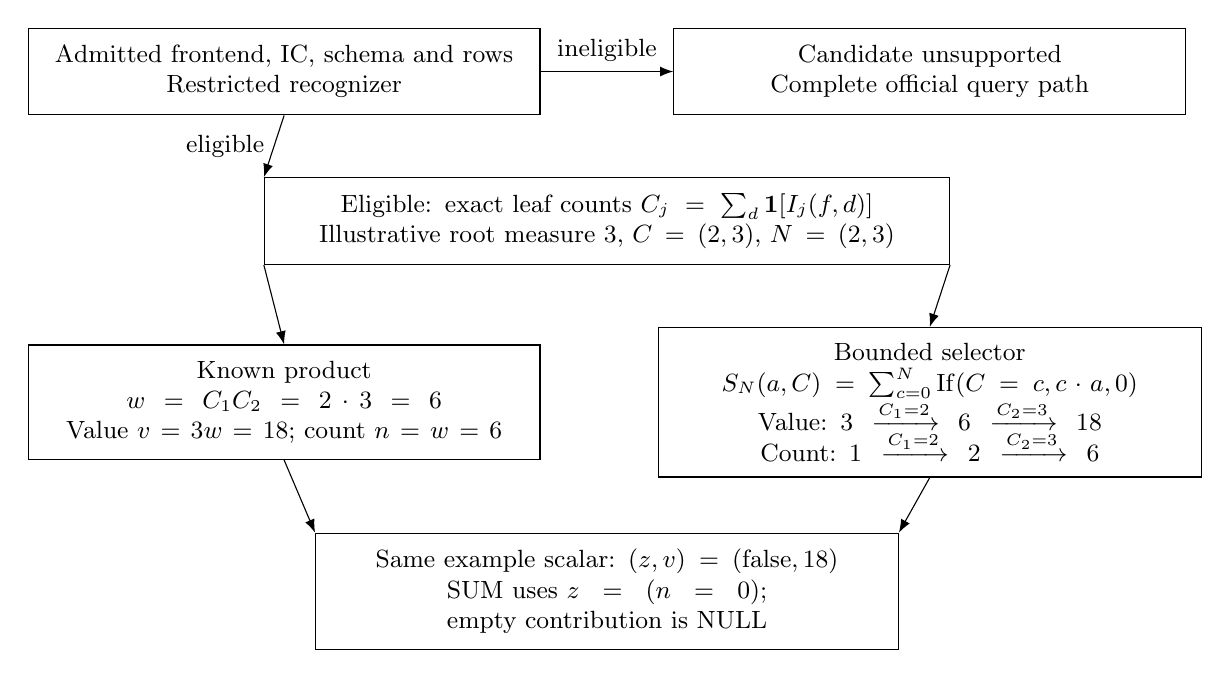
\begin{tikzpicture}[font=\small,>=Latex,
 box/.style={draw,align=center,minimum height=11mm,inner sep=2mm}]
\node[box,text width=61mm] (rec) at (-41mm,0)
 {Admitted frontend, IC, schema and rows\\Restricted recognizer};
\node[box,text width=61mm] (official) at (41mm,0)
 {Candidate unsupported\\Complete official query path};
\node[box,text width=83mm] (counts) at (0,-19mm)
 {Eligible: exact leaf counts $C_j=\sum_d\ind{I_j(f,d)}$\\Illustrative root measure $3$, $C=(2,3)$, $N=(2,3)$};
\node[box,text width=61mm] (product) at (-41mm,-42mm)
 {Known product\\$w=C_1C_2=2\cdot3=6$\\Value $v=3w=18$; count $n=w=6$};
\node[box,text width=65mm] (selector) at (41mm,-42mm)
 {Bounded selector\\$S_N(a,C)=\sum_{c=0}^{N}\ite(C=c,c\cdot a,0)$\\Value: $3\xrightarrow{C_1=2}6\xrightarrow{C_2=3}18$\\Count: $1\xrightarrow{C_1=2}2\xrightarrow{C_2=3}6$};
\node[box,text width=70mm] (scalar) at (0,-66mm)
 {Same example scalar: $(z,v)=(\mathrm{false},18)$\\SUM uses $z=(n=0)$; empty contribution is NULL};
\draw[->] (rec)--node[above]{ineligible}(official);
\draw[->] (rec.south)--node[left]{eligible}(counts.north west);
\draw[->] (counts.south west)--(product.north);
\draw[->] (counts.south east)--(selector.north);
\draw[->] (product.south)--(scalar.north west);
\draw[->] (selector.south)--(scalar.north east);
\end{tikzpicture}
\caption{Alternative encodings for one illustrative, non-NULL root value with $R(f)=\mathrm{true}$. Exact $C_j$ counts actual leaf positions with TRUE predicates, not free variables. The leaf sizes/count bounds $N=(2,3)$ are illustrative, not the executed two-leaf/two-row setup. Product and selector produce the same SUM value and non-NULL contribution count; local flat enumerates six joined positions. NULL arguments contribute nothing, and zero contributions yield NULL SUM. Unsafe frontend normalization or an unverified IC stops before both routes; only candidate ineligibility uses the official fallback. The example supplies no measured cost or speed claim. The editable TikZ layout was prepared with OpenAI Codex assistance; its original model version was not retained. No generated bitmap is used.}\label{fig:interface}
\end{figure}

% Method statements; measured outcomes are separately reported in results_current.tex.
\subsection{A common source-AST contract bridge}\label{sec:bridge}
The direction failure in Section~\ref{sec:icdiagnostic} motivates a common adapter before any comparison arm. Its accepted IC AST is absent or a conjunction list, allowing nested AND, non-NULL tests, one column compared with one integer literal in either order using six comparison operators, and inclusive column BETWEEN integer bounds. Every clause must be TRUE on every physical row of its referenced table; NULL fails. This explicit contract is narrower than the upstream interface and does not infer SQL CHECK semantics. One unsupported node refuses the whole contract without fallback.

Let $B$ be the fresh Environment's schema, exact-row facts and bounds before adding the tested IC. A separate reference emits $C_r$ from the original AST on the same base symbols. A normalized copy reverses literal-left ordered comparisons and expands BETWEEN into inclusive column-left bounds; only this copy enters the actual upstream compiler, whose added facts form $C_u$. Original AST and per-leaf transformations are retained. Admission requires
\begin{equation}
\operatorname{SAT}(B),\qquad
\operatorname{UNSAT}\bigl(B\land(C_u\mathbin{\oplus}C_r)\bigr).
\label{eq:bridge}
\end{equation}
Neither tested interpretation is asserted in the XOR premises, where it could hide mapping counterexamples. For the XOR audit, SAT or unknown refuses admission. Base SAT prevents a vacuous audit; a separate later guard requires $B\land C_u$ satisfiable and excludes deleted rows. Contradictory ICs are not query-equivalence successes.

Every arm audits the same registered IC in a fresh Environment. Fallback and differentials require its attached bridge record and unchanged complete-fact digest. These local identity checks are not portable certificates, and the official arm uses an explicitly controlled IC adapter. A concrete evaluator checks every SAT witness against the original AST before the integer-domain audit and unchanged SQL replay. All checks count toward the process budget.

Equation~\ref{eq:bridge} establishes bounded equality of the two interpretations, conditional on the base representation and reference implementation. The reference shares base variables and solver primitives but not the upstream IC compiler. This does not certify text parsing, arbitrary ICs, business truth or query translation. Executed audits are input-specific; old v4 runs inherit no bridge guarantee.


\subsection{Mapping obligations}\label{sec:mapping}
Constructed column pairs \texttt{V\$X}/\texttt{V\_DOLLAR\_X} and \texttt{A.B}/\texttt{A\_\_\_\_B} produced identical ASTs/plans although original SQL returned 2 and 7. No solver ran in these diagnostics: they expose lossy parsing, not an observed solver verdict. Ten later guarded slots rejected both cases before fallback; 35 unselected routing slots remain not run. An earlier six-slot name-mapping rejection is also retained.

Table~\ref{tab:mapping} maps definitions to code. Differentials check consistency, exact-row liveness, scalar shape, fresh definitions and NULL/value difference. Their common query encoding remains a trust boundary despite the separately audited IC AST.

\begin{table}[htbp]
\centering\small
\begin{tabularx}{\textwidth}{p{.18\textwidth}p{.27\textwidth}X}
\toprule
Object & Implementation & Boundary\\
\midrule
Fragment, $e$ & \texttt{recognize}, \texttt{value} & Root arithmetic, strict NULL; complete INT schema\\
$R,I_j$ & \texttt{true\_predicate} & TRUE-only atoms; no cross-leaf predicate\\
$C_j,M$ & \texttt{encode} & Exact row indicators and match-count products\\
Fresh definitions & Query/mode-specific prefix & Acyclic total definitions; differential checks\\
Scalar difference & \texttt{unequal} & NULL payload ignored; result row preserved\\
Contract AST & Common bridge + reference & Base SAT; contract XOR UNSAT; source AST only\\
Concrete witness & Original IC + domain + SQL & Original IC, integer domain, then raw SQL; common-plan oracle boundary\\
\bottomrule
\end{tabularx}
\caption{Definition-to-code map. Local checks do not promote the abstract lemmas into a theorem of the complete SQL implementation.}\label{tab:mapping}
\end{table}

\subsection{Concrete replay domain}\label{sec:oracle}
SMT uses mathematical integers; SQLite may promote overflowing expressions to REAL or reject overflowing SUM. Before replay, the common auditor checks base values, expression intermediates and weighted aggregates. For flattened associative expressions it bounds positive/negative addition totals and absolute nonzero products across parenthesizations; SUM is checked across row orders. Unsafe or unproved cases remain \texttt{UNKNOWN\_ORACLE\_DOMAIN}, without clipping, rounding or changed constraints. This conservative check can reject a safe concrete order. Only admitted witnesses replay the complete original SQL, preserving duplicates and NULL. The auditor shares the candidate plan and is not an independent semantic oracle.

All raw outcomes and separately derived acceptance categories retain their denominators. Contradictory contracts stop before query comparison; concrete replays and finite differentials do not prove parser totality or complete compiler correctness.

\section{Evaluation design}\label{sec:evaluation}
All cases are exposed development material, without held-out data or human gold. Six original cases cover conjunction order, nullable COUNT, non-NULL ICs, SUM/COUNT differences, empty SUM and all-NULL SUM. At two row bounds they give twelve configurations; ten v4 expression controls and six v5 IC-adapter controls yield 28 configurations but only 22 logical cases. Six cost arms register 168 slots; two queries times three encoders separately register 168 differential slots. These repetitions are not independent samples. V4 and v5 remain separate contract versions.

The six arms are official, official with generic SMT preprocessing, local flat, known product, selector, and official with cheap AND normalization. The last recursively sorts admitted conjunction operands: identical normalized ASTs give a conditional result; otherwise official fallback runs. It is not a full optimizer and shares the frontend boundary. Each arm uses a fresh process/Environment, common native library and complete input, CPU soft/hard limits of 14/15 seconds, a 25-second supervised wall limit and 1 GiB RSS limit. Startup, IC audits, all query work, fallback, replay and cleanup count toward cost. Solver threads are one; auxiliary monitoring threads exist. One pass does not establish statistical speedup.

Applicability covers 397 Calcite, 64 literature and 23,994 LeetCode pairs, retaining all 48,910 query slots and duplicates. The v4 recognizer consumes saved official ALL-dialect ASTs and errors. It does not reparse SQL, reconstruct missing ASTs, assert ICs, encode, solve or execute queries. This is a cached recognizer scan, not parser validation or equivalence accuracy. Original unequal-budget runs and fixed-point checks remain separate diagnostics.

\section{Results and retained failures}\label{sec:results}
% Frozen final v5 cut: 1d6d0291fda36937a26da6b46c9d07b18899a21686708fa4279c7a814e48b95c.
\subsection{Complete v5 outcomes}
Table~\ref{tab:v5outcomes} accounts for every selected slot. A strict query result requires the recorded bridge and full-contract gates, complete worker/cleanup receipts, acceptable process supervision and, for SAT, original-AST validation and safe original-SQL replay. Typed refusals remain separate from query decisions. These counts describe exposed development configurations, not independent benchmark accuracy.

\begin{table}[htbp]
\centering
\begin{tabular}{lrrrrrr}
\toprule
Run & Slots & Strict & Unknown & Domain & Typed & Monitor\\
\midrule
Six-arm cost & 168 & 127 & 7 & 6 & 24 & 4\\
Query differential & 168 & 115 & 23 & 0 & 24 & 6\\
SpotIt engine & 28 & 21 & 2 & 1 & 3 & 1\\
\bottomrule
\end{tabular}
\caption{Mutually exclusive v5 categories. Strict means a valid pair decision for cost/SpotIt, or bounded encoder agreement for differential. Domain denotes an unproved replay domain; Typed is a verified expected no-query refusal; Monitor is unavailable RSS observation, not established memory exhaustion. No failed category is an equivalence success.}\label{tab:v5outcomes}
\end{table}

The cost records contain 78 raw UNSAT, 52 SAT, eight unknown, six oracle-domain unknowns, eighteen refusals for inconsistent contracts and six for unsupported contracts. Four monitoring stops override raw outcomes: two SAT, one UNSAT and one unknown. Thus strict decisions are 77 UNSAT and 50 SAT, not all 130 raw decisions. All 52 stored SAT witnesses pass original-contract and SQL replay checks; the two monitored attempts remain excluded from strict results. Across the prior twelve configurations, ten arithmetic controls and six adapter controls, strict pair counts are respectively 62/72, 47/60 and 18/36; the last group also has eighteen valid typed refusals.

Recovery retains 169 cost attempts for 168 slots: terminal slot 51 comes from the old batch, resumed 52--53 from the new one. Interrupted 52 and the earlier not-run 53 remain recorded. Interrupted 52 lacks full cost; its 1.234-second CPU checkpoint is only a lower bound. Stale raw pair-work fields are preserved; separate start, final-phase, cleanup and reaped-process receipts derive execution state without turning unknown/monitored outcomes into success.

\subsection{Contract controls and differentials}
For each cost and differential campaign, 162 inputs record base-only SAT and contract-XOR UNSAT; the six unsupported-contract controls stop before either check. Eighteen admitted contracts are contradictory and stop before query work. These input-specific checks do not certify arbitrary contract translation. In D01, $5<T.A$ together with $T.A\le6$ forces the integer value 6: all six arms produce a strict SAT witness, validate the original AST and replay NULL versus 6. D02 yields six UNSAT decisions for an identical query; D03 yields six SAT decisions without explicit ICs. D04/D05 reject twelve inconsistent contracts, and D06 refuses six whole contracts containing an unsupported disjunction. All are constructed repair controls, not naturally collected defects.

Individual-query records contain 120 raw UNSAT differentials, 24 unknown and 24 typed refusals. Five raw UNSAT and one unknown coincide with monitoring stops, leaving 115 strict agreements. Flat, product and selector have respectively 39, 37 and 39 strict agreements out of 56 registered slots each. No validated differential counterexample is recorded, but the unknowns and refusals prevent a complete mapping result. These checks remain relative to shared query encoding and cannot replace the abstract premises with a general compiler theorem.

\subsection{Costs and comparison boundary}
Table~\ref{tab:v5cost} reports complete process costs for the 168 selected returned slots, including failures and refusals. The official arm also has an interrupted attempt whose full cost is unknown and is not included in these totals. Selector and flat totals are close, their strict counts differ, and each arm contributes one selected returned observation per configuration. No speedup, stability or selector-specific advantage follows.

\begin{table}[htbp]
\centering
\begin{tabular}{lrrrrr}
\toprule
Arm & Strict/28 & Unknown & Monitor & CPU sum (s) & Median (s)\\
\midrule
Official + IC adapter & 20 & 2 & 1 & 62.612 & 1.315\\
Official + generic SMT & 21 & 2 & 0 & 63.180 & 1.354\\
Local flat & 23 & 0 & 0 & 37.110 & 1.314\\
Known product & 19 & 3 & 1 & 73.661 & 1.336\\
Local selector & 22 & 0 & 1 & 36.793 & 1.333\\
Official + cheap AND & 22 & 0 & 1 & 50.485 & 1.332\\
\bottomrule
\end{tabular}
\caption{V5 cold-process CPU, 28 observed returns per arm. Each arm additionally has one domain refusal and four valid typed refusals. Official has a 29th, interrupted attempt with unrecorded full cost; its sum is incomplete campaign cost. Medians are across different outcome mixtures, not repeated trials.}\label{tab:v5cost}
\end{table}

For S01 at N4, official and generic-SMT return unknown; flat, selector and cheap AND return strict UNSAT at 1.314, 1.312 and 1.298 seconds CPU. Product records UNSAT at 1.361 seconds but has a monitoring stop and is not strict. Standard conjunction normalization therefore explains a success that cannot be uniquely attributed to selectors.

The controlled SpotIt engine selects 28 slots from its 168-slot enclosing manifest; 140 other-arm slots are unselected, not failures. Its 21 strict results comprise twelve UNSAT and nine replayed SAT. One raw inconsistent-contract refusal has a monitoring stop, leaving three valid typed refusals. CPU sums to 63.881 seconds. All 28 source-backed dispatch records identify AUTO\_SET with all-null deletion disabled. This uses reconstructed native Z3 4.12 despite outer requirements specifying 4.15 and does not reproduce the full SpotIt+ mining pipeline. Scalar one-row set/bag coincidence does not change the engine implementation. Polygon's search and precise modes remain unbenchmarked under a matched domain.

\subsection{Historical v4 and fixed-point evidence}
V4 separately records 72 UNSAT, 41 SAT, seven unknown and twelve refusals across 132 cost slots. Six contract refusals retain raw NOT\_RUN/BLOCKED\_OR\_ERROR. E01--E08's 48 decisions match expectations; eighteen SAT witnesses replay. Their 48 raw UNSAT differentials have three RSS-observation anomalies, versus one among 36 earlier v3 checks. These inherit no v5 bridge or strict-acceptance guarantee.

On twelve v4 configurations, flat/selector CPU was already close at 16.862/16.725 seconds with no unknowns. Product, official, generic and cheap AND took 52.130, 42.439, 42.410 and 30.133 seconds with 2, 2, 2 and 1 unknowns. Earlier N2 totals of 7.444--7.750 seconds also establish no selector advantage. Twelve fixed-point controls yield eighteen safe replays and three domain unknowns among 21 queries, not equivalence proofs. Historical SpotIt's 22 slots retain eleven UNSAT, seven SAT, two unknown, two refusals and an RSS anomaly. Full versioned records remain in the evidence package; they are not pooled replicates.

\subsection{Complete public applicability}
Table~\ref{tab:versionedcoverage} includes all 24,455 public pairs. The six eligible slots correspond to four exact SQL strings or five SQL/full-context combinations, all with zero leaves. The two both-eligible pairs are an identical Calcite SUM pair and a literature COUNT comparison over one relation. Eligible public JOIN coverage is therefore zero, and LeetCode has no eligible slot. Its 23,994 pairs span only 56 source problem labels and 24,050 distinct SQL strings, not 23,994 independent tasks.

\begin{table}[htbp]
\centering
\begin{tabular}{@{}lrrrrrr@{}}
\toprule
Source & Slots & Eligible & Ineligible & Refused & Unknown & Errors\\
\midrule
Calcite & 794 & 4 & 548 & 188 & 38 & 16\\
Literature & 128 & 2 & 125 & 0 & 0 & 1\\
LeetCode & 47,988 & 0 & 46,758 & 1 & 0 & 1,229\\
\midrule
Total & 48,910 & 6 & 47,431 & 189 & 38 & 1,246\\
\bottomrule
\end{tabular}
\caption{Full cached official ALL-AST scan using the v4 recognizer retained by v5. Refusals are raw frontend rejections; errors preserve original parse/AST-record failures. No slot is unprocessed. The scan does not execute the v5 IC bridge, reparse SQL or run a solver.}\label{tab:versionedcoverage}
\end{table}

No eligibility filter or deduplication reduces the denominator. Two LeetCode blocks stopped after 1,973 and 1,978 recorded slots; resumes processed only the remaining 27 and 22, preserving earlier hashes and resource stops. Thirty-eight Calcite slots become UNKNOWN because cached AST objects cannot be safely reconstructed. The v4 extension adds no eligible query over v3. At pair level, two are both eligible, 24,412 definitively ineligible and 41 unresolved. This is applicability, not public equivalence accuracy.

Earlier 922-slot scans admit seven queries under v2/MYSQL and v2/ALL, versus six under guarded v3; these configuration changes are not independent tests. Static inventories found no original-fragment member among TPC-H's 22, SSB's thirteen or DuckDB TPC-DS's 99 definitions; official TPC-DS SQL was unavailable. Three SSB definitions became structural candidates only under combined arithmetic/BETWEEN/domain changes, each with one leaf. These static checks are not solver runs and provide no executed public join case.

\subsection{Constraint-direction counterexample}\label{sec:icdiagnostic}
A constructed diagnostic evaluates six literal-left operators at four values, including NULL: eight of its 24 cells disagree with the emitted official constraint. In particular, $5<T.A$ is emitted in the opposite direction. With one exact row, the official checker reports UNSAT for \texttt{SUM(T.A) WHERE T.A<5} versus unfiltered \texttt{SUM(T.A)}. Yet the original contract admits $T.A=6$, for which unchanged SQL returns NULL versus 6 in SQLite. This is an observed false-equivalence result under the original contract. The cells include fixed-model and substitution controls, not 24 independent verification problems or a defect-frequency estimate. V5's narrow AST adapter and D01 address this constructed direction error; they do not retroactively certify v4, arbitrary ICs or business truth.


\section{Natural-query development diagnostics}\label{sec:natural}
\subsection{Source and selection protocol}
The zero-join admission result in Table~\ref{tab:versionedcoverage} concerns the original cached recognizer and its narrow language; no solver ran in that scan. It therefore cannot be explained as a solver timeout. In particular, whole-schema INT restrictions and the exclusions of DISTINCT, grouping and mixed-type expressions block queries before candidate encoding. Relaxing a parser guard alone does not establish the premises of the factorization lemmas.

We separately inspect a frozen ParSEval artifact \citep{chen2025parseval}: 1,534 records at source commit \texttt{88cfe245}, official run 37547685455, artifact 11452059162. The selection retains the previously observed pair 1172 and adds three pairs from each official EQ, NEQ and unresolved stratum. Unresolved includes UNKNOWN, TIMEOUT and SYNTAX\_ERROR. A lexical JOIN and aggregate-token screen is followed by ranking the SHA-256 hash of a UTF-8 string containing the prefix \texttt{cg-boundary09-v1}, database identifier and pair index, separated by vertical bars, exact unordered-pair deduplication and a maximum of two cases per database, applied in stratum order. There is no outcome-driven refill. Semantic duplicates are not ruled out. This is a diagnostic sample, not a population estimator: the anchor and an earlier aggregate-DISTINCT summary were already inspected, and all extracted records are exposed development material.

Table~\ref{tab:natural} preserves all ten selected pairs. Original source SQL and all source DDL are retained. ``Full contract'' here means those registered source constraints, not unstated business rules or a universal proof of SQLite type fidelity. This later contract includes foreign keys and differs from the original v5 AST contract. We do not pool their results or costs.

\begin{table}[htbp]
\centering\small
\begin{tabularx}{\textwidth}{r l r X}
\toprule
Pair & Source database & Tables/columns & Final diagnostic status\\
\midrule
750 & superhero & 10/31 & Polygon: concrete NEQ in both modes\\
319 & toxicology & 4/11 & Polygon: bounded UNSAT in both modes; identical SQL\\
1172 & thrombosis & 3/64 & Polygon with local observation adapter: concrete NEQ\\
1261 & thrombosis & 3/64 & Polygon with separate RF adapter: bounded UNSAT\\
1073 & football & 7/199 & Not admitted to Polygon; two SQLite distinguishing databases\\
45 & california & 3/89 & Not admitted to Polygon; four SQLite distinguishing databases\\
1526 & debit\_card & 5/21 & Not admitted to Polygon; two SQLite distinguishing databases\\
1490 & debit\_card & 5/21 & Not admitted; static rewrite analysis only, no solver result\\
26 & california & 3/89 & Invalid predicted SQL: unresolved \texttt{T1.Street}\\
1390 & student\_club & 8/48 & Invalid predicted SQL: unresolved \texttt{T2.link\_to\_event}\\
\bottomrule
\end{tabularx}
\caption{The complete ten-pair development inventory. Four of eight syntactically valid pairs reach the adapted Polygon experiment. The other four are not counted as solver failures; the two invalid inputs remain in the ten-pair denominator.}\label{tab:natural}
\end{table}

\subsection{Sampled testing and bounded symbolic search}
For pair 1172, both source queries count distinct patient IDs after joining Patient to Laboratory and selecting male patients. The gold query tests \texttt{T-BIL} $\ge 2.0$; the predicted query tests $>2.0$. One official ParSEval call returned EQ. All nine saved candidate databases satisfy the source contract and yield equal outputs on independent replay. A separate valid three-table control with a male patient and laboratory TBIL value 2 yields 1 versus 0. The generated candidates do not isolate this difference: other qualifying rows can mask it under DISTINCT. This is one exposed diagnostic, not a measured error rate or a proof of a unique causal mechanism. Our first post-call replay worker raised a case-sensitive \texttt{Patient} lookup error. That local error remains recorded and is not attributed to ParSEval. An independent reader replayed the saved candidates and control without rerunning the baseline or using the control as a generation seed.

We subsequently execute Polygon commit \texttt{5e182373} in under-approximation (UA) and precise modes on four admitted pairs. The serial resource adapter changes the per-call limit from 300 seconds to 3 seconds, also caps UA solver calls at 3 seconds, sets each Z3 call's internal memory limit to 512 MiB, and enforces a 12-second worker limit and 60-second batch limit. Per-call memory is not aggregate resident memory. All owned process handles were reaped. Python 3.12, Z3 4.16.0 and SQLite 3.53.3 differ from the original v5 setup; these are short adapted diagnostics, not a reproduction of Polygon's published timings.

\begin{table}[htbp]
\centering\small
\begin{tabular}{r l rr rr}
\toprule
 & & \multicolumn{2}{c}{UA} & \multicolumn{2}{c}{Precise}\\
Pair & Outcome in each mode & Wall seconds & Z3 calls & Wall seconds & Z3 calls\\
\midrule
750 & Validated NEQ & 0.816278 & 2 & 0.587529 & 1\\
319 & Bounded UNSAT & 0.434618 & 3 & 0.409159 & 1\\
1172 & Validated NEQ & 0.891738 & 2 & 0.399413 & 1\\
1261 & Bounded UNSAT & 0.951991 & 3 & 0.369814 & 1\\
\bottomrule
\end{tabular}
\caption{Eight completed Polygon slots at at most one row per source table, with 14 Z3 calls. Times are single worker-wall observations including local setup and checks; they are not comparable to the v5 CPU table and do not establish a speed ranking.}\label{tab:polygon}
\end{table}

Pair 750 has eight primary-key, eight NOT NULL and eleven foreign-key constraints. Its concrete outputs are NULL versus $-54.0$ in UA and $-55.0$ versus NULL in precise mode. Negative values satisfy the source DDL; we do not infer business plausibility. Pair 319 has four primary-key, five NOT NULL and five foreign-key constraints and byte-identical SQL. Its bounded UNSAT result supplies no distinguishing witness.

Pairs 1172 and 1261 retain the three-table, 64-column schema and its two primary-key, three NOT NULL and two foreign-key constraints. They use separate source-specific observation adapters at $N\le1$. For 1172, TBIL classes preserve NULL and the relevant comparison outcomes using NULL, 0.0, 2.0 and 3.0 representatives; sex classes preserve the male test. Pair 1261 instead preserves the RF TEXT comparison with 20 and Thrombosis comparison with 0. These are manually checked, query-specific classes, not a generic SQLite abstraction. An abstract candidate must satisfy the encoded contract before a fixed lift; the original contract and SQL are then checked without repairing an invalid model. Both 1172 modes lift to the same concrete 1-versus-0 witness, hence do not constitute two independent failures. For 1261, an intermediate UA SAT assignment lacks the required full join/filter match and is not a counterexample. Completed searches return bounded UNSAT. No argument establishes unbounded equivalence or a complete implementation theorem.

These observations defeat the motivation that existing strong symbolic methods cannot handle the selected cases. They do not establish broad Polygon coverage: four valid pairs remain outside the admitted local contract, and two selected inputs are invalid.

\subsection{SQLite witnesses outside the admitted symbolic contract}
Eight constructed databases distinguish three of the remaining source pairs (Table~\ref{tab:sqlite}). Each was checked against the complete original DDL and registered constraints, and both original SQL strings were replayed independently. They are synthetic witnesses for natural query pairs, not naturally occurring database defects, official test databases, or Polygon solver successes. No exhaustive minimality or business-realism claim is made. Pair 1490 remains a static IIF/CASE and non-NULL COUNT rewrite analysis; it has no new dynamic equivalence result. The competing source-date interpretations for 1526 remain unresolved.

\begin{table}[htbp]
\centering\small
\begin{tabularx}{\textwidth}{r l rr X}
\toprule
Pair & Distinguishing condition & $N$ & Rows & Output difference\\
\midrule
1073 & Invalid date conversion & 1 & 2 & 1 versus 0\\
1073 & Nullable INT primary key & 1 & 2 & 0 versus 1\\
45 & Text numeric coercion & 1 & 2 & $(S,\texttt{x})$ versus $(S,0.0)$\\
45 & Large integer and REAL & 1 & 2 & 9007199254740993 versus 9007199254740992.0\\
45 & Group merging & 2 & 4 & $(S,1),(S,3)$ versus $(S,2.0)$\\
45 & Output bag multiplicity & 2 & 4 & Two copies of $(S,0)$ versus one of $(S,0.0)$\\
1526 & Empty scalar contribution & 1 & 4 & 1.0 versus NULL\\
1526 & SUM and scalar scope & 3 & 7 & 0.8333333333333334 versus 0.5\\
\bottomrule
\end{tabularx}
\caption{Eight SQLite witnesses across three exposed query pairs. $N$ is the largest table cardinality in that concrete database; Rows is the total over all source tables. The short output descriptions retain the values or multiplicities deciding inequality.}\label{tab:sqlite}
\end{table}

\subsection{COUNT repairs and implementation boundary}\label{sec:diagnosticimplementation}
Local diagnosis found three COUNT implementation issues in the pinned Polygon-based runtime. P1 uses integer indicators for ordinary COUNT(*); P2 extends the grouped COUNT(*) FILTER path; P3 resolves bare-column FILTER expressions at three parser entry points. These are engineering repairs. The same 42 exposed regressions comprise 28 concrete parser-expression cases and 14 concrete FProject/FGroupBy operator-chain cases, including NULL, deleted slots, filters and grouping. They evaluate concrete symbolic expressions without starting a solver or the complete QueryEncoder/Environment pipeline.

\begin{table}[htbp]
\centering\small
\begin{tabular}{l rrr rrr}
\toprule
 & \multicolumn{3}{c}{28 expression cases} & \multicolumn{3}{c}{14 operator-chain cases}\\
Version & Pass & Mismatch & Error & Pass & Mismatch & Error\\
\midrule
Original & 12 & 4 & 12 & 7 & 6 & 1\\
P1 & 28 & 0 & 0 & 9 & 5 & 0\\
P2 & 28 & 0 & 0 & 11 & 3 & 0\\
P3 & 28 & 0 & 0 & 14 & 0 & 0\\
\bottomrule
\end{tabular}
\caption{Fixed-development regression results for successive COUNT repairs. Independent SQLite and separate Python references checked all 168 saved records; that review did not rerun Polygon's encoder. Passing P3 does not prove arbitrary FILTER or aggregate semantics.}\label{tab:countrepair}
\end{table}

The successful local regression execution used 0.847168 seconds across three segments, with zero solver calls and a reported process RSS of 60,489,728 bytes. Earlier Python-version and harness errors remain in the attempt record. One unused review-helper file changed before the final review-ready freeze; this preservation exception is disclosed rather than erased. The final 003 snapshot's 541 checked file hashes match. The independent result check is a recomputation of known development observations, not a held-out test. The three specific repairs do not affect the AVG or DISTINCT forms in the four earlier Polygon pairs; this impact analysis does not certify the rest of the baseline.

OpenAI Codex assisted with adapters, regression code, concrete witness construction, local execution and analysis. Independent AI agents inspected source contracts and replay records; their roles and prior involvement are retained in the local evidence ledger. No human gold labels, independent final test, model training or new experiment in the manuscript-integration phase is claimed.

\subsection{What the combined evidence establishes}
The abstract multiplicity equations and finite selector are known constructions, and the six-arm experiment does not establish a selector advantage. The public scan measures a frontend admission boundary rather than search cost. The natural-query inventory then distinguishes invalid inputs, unsupported semantics, concrete refutations and bounded UNSAT. Existing Polygon modes resolve the admitted examples; the remaining SQLite witnesses expose semantic obligations rather than a demonstrated missing search mechanism. Query-specific value classes and COUNT repairs cannot, by themselves, supply an original abstraction method. The evidence is consequently a restricted implementation study and a set of traceable diagnostics; a generalizable new algorithm or benefit remains unestablished.


\section{Limitations, lineage, and reproducibility}
\paragraph{Guarantees and lineage}
The lemmas cover the stated finite relational fragment, excluding general grouping, outer joins, cross-leaf filters and unbounded equivalence. The original v5 IC adapter excludes foreign keys and functional dependencies and does not infer business intent, authorization or temporal correctness. Exact-row and at-most-row domains differ. Post-hoc fragment changes require new versioned evidence; known factorization and simple preprocessing remain essential controls.

Historical governance prompting scored 156/159 against CaliberGraph's 147/159; a dbt-derived result tied at 122/122 only with longest-alias linking, versus 120/122 for another linker. These do not evaluate this module. The legacy 1,108 distinct SQL attempts contain 1,074 connection/query timeouts and 34 cached first scalars; without complete same-snapshot references, all 1,488 model records remain semantically unknown, not 34/1,108 accuracy. No new business gold or human annotation is inferred.

The author states that this contribution does not duplicate SIGMOD847. Its inspected formal materials concern typed-delta refresh, reuse and version-consistent switchover. We do not borrow its algorithms, proofs or experimental numbers; ordinary additive aggregation and typed certificates are shared background. This records the author statement and inspected distinction, not an exhaustive originality proof.

\paragraph{Evidence}
The local package retains original inputs, raw reports and decoded databases, with hashes, interrupted attempts and complete denominators. A claim ledger links paper values to saved rows. No live production system, external model API or GPU was used for this manuscript task; local historical artifacts were read. Third-party source identities remain recorded; the package is not a public release.

\paragraph{Use of generative AI tools}
OpenAI Codex was used for code generation and repair, mathematical drafting, local experiment execution and orchestration, evidence analysis, manuscript preparation and the editable method diagram. The current independent review used GPT-6-astra with high reasoning effort; exact model versions for all earlier assistance were not retained. The experimental roles are also described in Section~\ref{sec:diagnosticimplementation}. Separate AI-agent review is not human peer review or an independent test set. This author-review candidate does not assert that the human authors have completed technical verification or approved submission. Those confirmations, complete tool-version records where recoverable, affiliations, correspondence, contributions, funding and conflict declarations remain outstanding. The historical author order is Hongsheng Wang, then Dazhen Deng. Author responsibility cannot be delegated to an AI tool.

\section{Conclusion}
CaliberGraph implements known factorization and bounded selectors for a restricted scalar language. Abstract identities, IC audits, differentials and replays cover distinct conditional guarantees. The controlled comparison establishes no selector benefit. The separate natural-query diagnostics show that existing symbolic search handles some cases missed by sampled testing, while SQLite typing, grouping and parser details remain distinct admission and implementation issues. These observations motivate careful contracts and failure accounting, but the exposed development evidence does not establish a new mechanism or a generalizable comparative benefit.

\bibliographystyle{elsarticle-harv}
\bibliography{references}
\end{document}
